%%%%%%%%%%%%%%%%%%%%%%%%%%%%%%%%%%%%%%%%%%%%%%%%%%%%%%%%%%%%%%%%%%%%%%%%%%%%%%%%
\documentclass[twocolumn]{revtex4}

%%%%%%%%%%%%%%%%%%%%%%%%%%%%%%%%%%%%%%%%%%%%%%%%%%%%%%%%%%%%%%%%%%%%%%%%%%%%%%%%
% Note that comments begin with a "%" and are not turned into text in the .pdf
% document.
%%%%%%%%%%%%%%%%%%%%%%%%%%%%%%%%%%%%%%%%%%%%%%%%%%%%%%%%%%%%%%%%%%%%%%%%%%%%%%%%

%%%%%%%%%%%%%%%%%%%%%%%%%%%%%%%%%%%%%%%%%%%%%%%%%%%%%%%%%%%%%%%%%%%%%%%%%%%%%%%%
% Include some extra packages.
%%%%%%%%%%%%%%%%%%%%%%%%%%%%%%%%%%%%%%%%%%%%%%%%%%%%%%%%%%%%%%%%%%%%%%%%%%%%%%%%
\usepackage[]{graphicx}
%%%%%%%%%%%%%%%%%%%%%%%%%%%%%%%%%%%%%%%%%%%%%%%%%%%%%%%%%%%%%%%%%%%%%%%%%%%%%%%%

%%%%%%%%%%%%%%%%%%%%%%%%%%%%%%%%%%%%%%%%%%%%%%%%%%%%%%%%%%%%%%%%%%%%%%%%%%%%%%%%
\begin{document}

%%%%%%%%%%%%%%%%%%%%%%%%%%%%%%%%%%%%%%%%%%%%%%%%%%%%%%%%%%%%%%%%%%%%%%%%%%%%%%%%
\title{
Can You Escape A Raptor Attack?
}

\author{C.~Stillman}
\author{M.~Bellis}
\affiliation{Siena College, Loudonville, NY}

\date{December 9th, 2015}

\begin{abstract}
	This project was designed to test our knowledge of a few programs we learned during our time in CSIS 200. The question at hand was: can you escape a raptor attack given a head start? The initial analysis was done on python. It was used to see if we could survive a raptor attack. For each part of the question I used varied python codes and functions. The results of this section were that you have a roughly 63.5 percent chance of surviving. My code was designed so that you could plug in any velocity equations and calculate the point of intersection and when the raptor is one meter behind.The second part of the project was too write up the results on a latex document as I am doing now. The third and final part was to upload using GIT. I used git commit and git push to push each part of my project to a repository on github. 
    	
\end{abstract}

\maketitle
%%%%%%%%%%%%%%%%%%%%%%%%%%%%%%%%%%%%%%%%%%%%%%%%%%%%%%%%%%%%%%%%%%%%%%%%%%%%%%%%

%%%%%%%%%%%%%%%%%%%%%%%%%%%%%%%%%%%%%%%%%%%%%%%%%%%%%%%%%%%%%%%%%%%%%%%%%%%%%%%%
\section{Introduction}
In this section I will outline the procedure used to achieve my results.
	The procedure for the first part was done using lines of python code in the Ipython notebook. The first question was done using a sub function of python: graphing. Once I created a graph I used a function to take in the distance and time values for each partisan. I had it output when they had traveled the same distance and how far the human traveled in that amount of time. The next section I used the same function but instead set up an inequality that when less then 1 it out put the new time. This was to determine how far and in how much time the raptor was exactly 1 meter behind the human. The final part of the question was about probability. I used a random number generator from numpy to create a number between 0 and 1. I then used each probability as a decimal. I compared that decimal to a random number and if the random number was outside the decimal the human dodged a chomp from the raptor. I did this with each respective probability except if it passed the first it moved onto the second and then onto the third. If it dodged all three the human lived! To calculate the probability I took the number of successful attempts and divided that by the number of attempts made. I got a 64 percent rate!
%%%%%%%%%%%%%%%%%%%%%%%%%%%%%%%%%%%%%%%%%%%%%%%%%%%%%%%%%%%%%%%%%%%%%%%%%%%%%%%%


%%%%%%%%%%%%%%%%%%%%%%%%%%%%%%%%%%%%%%%%%%%%%%%%%%%%%%%%%%%%%%%%%%%%%%%%%%%%%%%%
\section{Position vs. time}
	The first part of the assignment was to make a position vs time graph of the raptor and a human. Position can be given as $x = vt + x_i $ or velocity over time plus the initial position. The raptor's position can be described as  $x = 18(m/s)t $, or its velocity per second equals its position. The humans position can be shown as $ x = 3(m/s)t + 30 $, or his velocity per second plus 30 initial meters (being a slight head start). To make a position vs time graph I used matplotlib. To create a graph I entered some plots using the command plt.plot. I used this line twice as there are two seperate velocity equations. I set my x axis limit and y axis limit to include enough time and distance to show where they intersect. I used a few more lines of code such as plt.legend to add a legend and plt.title to add an appropriate title to my graph. The human had a little head start though so the raptor must overcome that distance and whatever distance the human traveled in order to eat him.
	\begin{figure}[h]
	\centering
	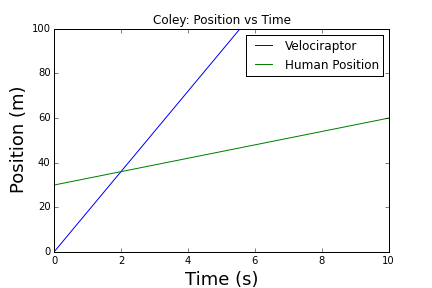
\includegraphics[scale=.5]{Position_vs_Time.png}
	\caption{My position vs time graph for the raptor and human}
	\end{figure}
\section{When does the raptor catch up to you?}
	To determine when the raptor catches up to you I made a python function that took in three variables. It took in the two position equations (the raptors and humans) and time. Within the function I set the two position equations equal to each other ($ 18(m/s)t = 3(m/s)t + 30 $) for any x value in the range 0 to 10000. The reason my x range is 0 to 10000 is because I needed to generate enough time instances to include the time where they crossed. By making a linspace you don't guarentee that every number between whatever limit you set will be generated. My function was used to determine at what distance the raptor was on top of the human. From there I returned the values time and human distance minus 30 to account for the initial head start. This gave me two answers, 2 seconds and 6 meters. Two seconds being how long it took for them to collide and 6 meters being how far the human traveled in that amount of time. 
\section{When is it close enough to strike?}
	This next section asked to find when the raptor was one meter behind the human, which is its striking distance. To do this section I created the same general function where it took in the two position equations and time. From there I set my input range as to include 0 up to 10000 like above. This time it was more important to create enough x values as the time value will not be an integer. I knew it would be some decimal slightly below 2 seconds. After setting my range I created an if statement again but instead of being equal I made it that if the difference of the raptor and human distance is less then 1 return the time where that initially happens ($ 18(m/s)t - 3(m/s)t + 30 < 1 $). That gives me the exact time when the raptor is precisely behind the human which came out to be 1.93 seconds. The function also returned the humans distance minus 30 again to account for the head start. The human ended up running only 5.8 meters. Below is a graph with a line showing where they are one meter apart. I created the line using the time value calculated above. I made sure to not hard code it so given any situation you could show where anything is one meter apart. 
	\begin{figure}[h]
	\centering
	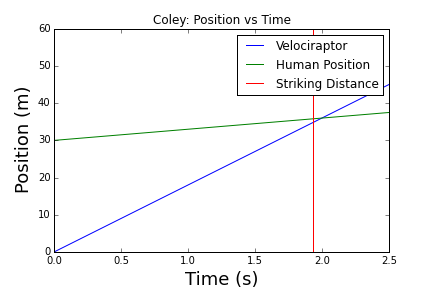
\includegraphics[scale=.5]{Position_vs_Time_Striking.png}
	\caption{My position vs time graph for the raptor and human}
	\end{figure}
	
\section{Will it bite you?}
	This section asked you to find the probability of the human escaping. To do this I used a random number generator from numpy (numerical python). I generated a random number between 0 and 1. I set this random number into a for loop that generated 1000 random numbers. Within this for loop I created an if loop. The if loop took each random number and separately ran them through a three stage set of if loops. The first tested to see if the number was greater then 0.2 representing 20 percent. The second if used 0.15 to represent 15 percent. The third if tested to see if the number was greater then 0.07 representing 7 percent. Within each if loop I had python generate a new random number as your odds reset after making it through each probability. If the random number was greater then each percent chance of failure I had it add a number 1 to an empty variable representing number of successful escape attempts. After 1000 random numbers were put through and reset each time It gave me a number around 0.645. I then put this number over 1000 $ p = s/x $ where p is probability, s is number of successful attempts, and x is number of trials. This number times 100 gives you your percent chance of success. The number I got was on average 63.5 percent. 
	
\section{Conclusion}
	The overall results of the process was that: given the situation you have approximately a 63 percent chance of surviving the raptor attack. These are surprisingly high odds granted the raptor was on you in a matter of seconds. The head start didn't do much in defense. Thankfully you are good at dodging raptor attacks and the raptor gets more and more inaccurate as its rage builds up. It is still an odd I wouldn't play with much, I have little interest in being raptor food. 

%%%%%%%%%%%%%%%%%%%%%%%%%%%%%%%%%%%%%%%%%%%%%%%%%%%%%%%%%%%%%%%%%%%%%%%%%%%%%%%%

%%%%%%%%%%%%%%%%%%%%%%%%%%%%%%%%%%%%%%%%%%%%%%%%%%%%%%%%%%%%%%%%%%%%%%%%%%%%%%%%
\end{document}
%%%%%%%%%%%%%%%%%%%%%%%%%%%%%%%%%%%%%%%%%%%%%%%%%%%%%%%%%%%%%%%%%%%%%%%%%%%%%%%%
